\documentclass[11pt]{extarticle}
\usepackage{amsmath, amssymb, amsthm, latexsym, amsfonts, indentfirst, xcolor, mathtools, manfnt, microtype}
\usepackage[utf8]{inputenc}
\usepackage{tikz}
\usetikzlibrary{decorations.pathreplacing,calligraphy}
\usetikzlibrary{shapes.geometric}

\begin{document}

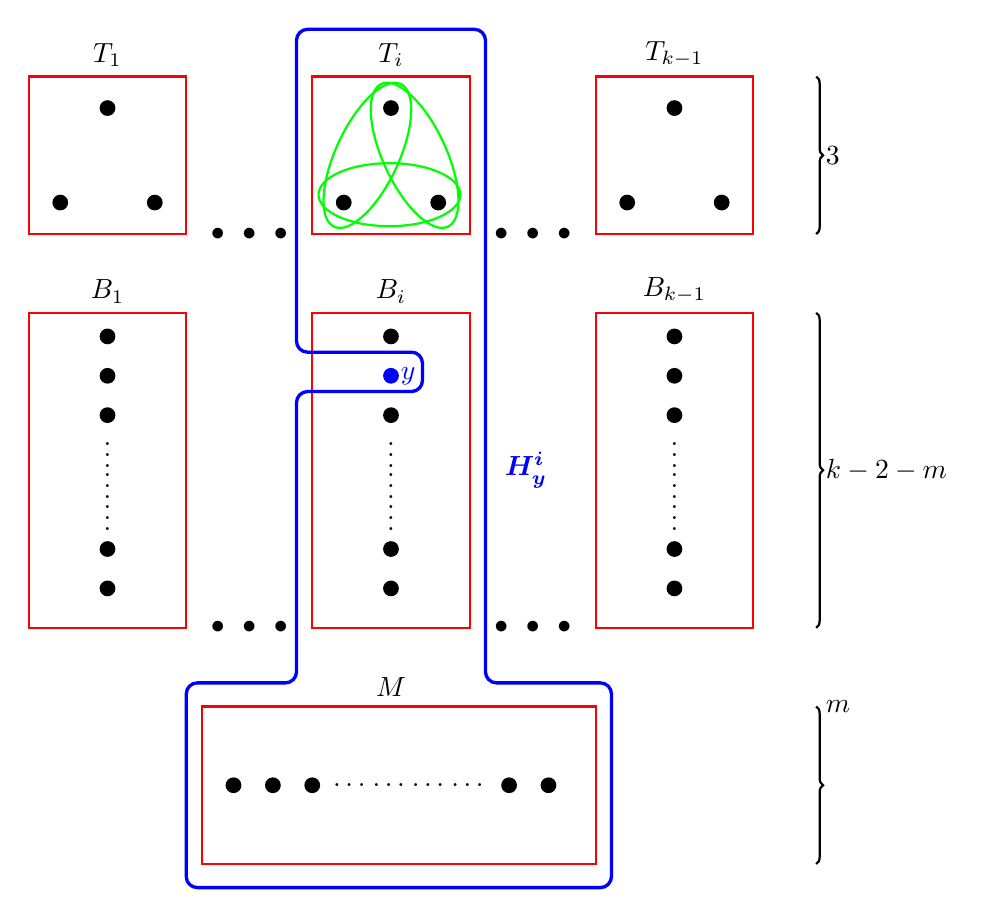
\begin{tikzpicture}
\coordinate (S) at (2, 2) ;
\coordinate (A) at (3.6, 0) ;
\coordinate (B) at (7.2,0) ;
\draw[thick, red] (0,0) rectangle (S);
\draw (1, 2) node[above] {$T_1$};

\fill[black] (0.4, 0.4)++(B) circle (0.1);
\fill[black] (1.6, 0.4)++(B) circle (0.1);
\fill[black] (1, 1.6)++(B) circle (0.1);

\fill[black] (0.4, 0.4)++(A) circle (0.1);
\fill[black] (1.6, 0.4)++(A) circle (0.1);
\fill[black] (1, 1.6)++(A) circle (0.1);

\fill[black] (0.4, 0.4) circle (0.1);
\fill[black] (1.6, 0.4) circle (0.1);
\fill[black] (1, 1.6) circle (0.1);

\node[ellipse, draw, color = green, thick, minimum width = 2cm, 
	minimum height = 0.8cm, rotate=65] at (4.3, 1) {};
\node[ellipse, draw, color = green, thick, minimum width = 2cm, 
	minimum height = 0.8cm, rotate=115] (e) at (4.9, 1) {};
\node[ellipse, draw, color = green, thick, minimum width = 1.8cm, 
	minimum height = 0.8cm] (e) at (4.58, 0.5) {};

\draw foreach \x in {1, 2, 3}
{ (2, 0)++(0.4*\x, 0) node {$\bullet$}};

\draw[thick, red] (A) rectangle ++(S);
\draw (A)++(1, 2) node[above] {$T_i$};

\draw foreach \x in {1, 2, 3}
{ (A)++(2 + 0.4*\x, 0) node {$\bullet$}};

\draw[thick, red] (B) rectangle ++(S);
\draw (B)++(1, 2) node[above] {$T_{k-1}$};

\coordinate (S`) at (2, -4);

\draw[thick, red] (0,-1) rectangle ++(S`);
\draw (1, -1) node[above] {$B_1$};

\draw foreach \x in {1, 2, 3}
{ (2, -5)++(0.4*\x, 0) node {$\bullet$}};

\draw[thick, red] (3.6, -1) rectangle ++(S`);
\draw (4.6, -1) node[above] {$B_i$};

\fill[black] (4.6, -1.3) circle (0.1);
\fill[blue] (4.6, -1.8) circle (0.1);
\draw[blue] (4.6, -1.8) node[right] {$y$};
\fill[black] (4.6, -2.3) circle (0.1);
\node at (4.6, -2.7) {\vdots};
\node at (4.6, -3.1) {\vdots};
\node at (4.6, -3.5) {\vdots};
\fill[black] (4.6, -4) circle (0.1);
\fill[black] (4.6, -4.5) circle (0.1);

\fill[black] (1, -1.3) circle (0.1);
\fill[black] (1, -1.8) circle (0.1);
\fill[black] (1, -2.3) circle (0.1);
\node at (1, -2.7) {\vdots};
\node at (1, -3.1) {\vdots};
\node at (1, -3.5) {\vdots};
\fill[black] (1, -4) circle (0.1);
\fill[black] (1, -4.5) circle (0.1);

\fill[black] (8.2, -1.3) circle (0.1);
\fill[black] (8.2, -1.8) circle (0.1);
\fill[black] (8.2, -2.3) circle (0.1);
\node at (8.2, -2.7) {\vdots};
\node at (8.2, -3.1) {\vdots};
\node at (8.2, -3.5) {\vdots};
\fill[black] (8.2, -4) circle (0.1);
\fill[black] (8.2, -4.5) circle (0.1);

\draw foreach \x in {1, 2, 3}
{ (5.6, -5)++(0.4*\x, 0) node {$\bullet$}};

\draw[thick, red] (7.2, -1) rectangle ++(S`);
\draw (8.2, -1) node[above] {$B_{k-1}$};

\draw[thick, red] (7.2, -6) rectangle ++(-5, -2);
\draw (4.6, -6) node[above] {$M$};

\draw [decorate,
	decoration = {brace, mirror}, thick] (10,0) --  (10,2);
\draw (10, 1) node[right] {$3$};
\draw [decorate,
	decoration = {brace}, thick] (10,-1) --  (10,-5);
\draw (10, -3) node[right] {$k-2-m$};
\draw [decorate,
	decoration = {brace}, thick] (10,-6) --  (10,-8);
\draw (10, -6) node[right] {$m$};

\draw [very thick, rounded corners, blue] (7.4, -5.7)--(7.4, -8.3)--(2,-8.3)--(2, -5.7)--(3.4, -5.7)--(3.4, -2)--(5, -2)--(5, -1.5)--(4.3, -1.5)--(3.4, -1.5)--(3.4, 2.6)--(5.8, 2.6)--(5.8, -5.7)--cycle;
\draw[ultra thick, blue] (5.9, -3) node[right] {$\boldsymbol{H_y^{i}}$};


\fill[black] (2.6, -7) circle (0.1);
\fill[black] (3.1, -7) circle (0.1);
\fill[black] (3.6, -7) circle (0.1);
\node at (4.1, -7) {\dots};
\node at (4.6, -7) {\dots};
\node at (5.1, -7) {\dots};
\node at (5.6, -7) {\dots};
\fill[black] (6.1, -7) circle (0.1);
\fill[black] (6.6, -7) circle (0.1);
 \end{tikzpicture}

\end{document}